\documentclass[conference,a4paper]{IEEEtran}

\usepackage{graphicx}
\usepackage{float}
\usepackage{amsmath}
\usepackage{booktabs}
\usepackage{stfloats}
\hyphenation{op-tical net-works semi-conduc-tor}

\DeclareRobustCommand*{\IEEEauthorrefmark}[1]{\raisebox{0pt}[0pt][0pt]{\textsuperscript{\footnotesize #1}}}

\begin{document}

\title{Rapid AI Drug Repurposing: A GraphSAGE-based Clinical Discovery Lab for Drug Repurposing on PrimeKG}

\author{
    \IEEEauthorblockN{
        Prathmesh Ojha\IEEEauthorrefmark{1}\IEEEauthorrefmark{*},
        Jhankar Bansal\IEEEauthorrefmark{1}
    }

    \IEEEauthorblockA{
        \IEEEauthorrefmark{1}
        Department of Computer Science and Engineering\\
        School of Engineering and Technology\\
        BML Munjal University, Gurugram, India\\
        prathmesh.ojha.23cse@bmu.edu.in,
        jhankar.bansal.23cse@bmu.edu.in
    }

    \IEEEauthorblockA{
        \IEEEauthorrefmark{*}Corresponding Author
    }
}

\maketitle

\begin{abstract}
Drug discovery is traditionally a time-intensive and resource-intensive process with high failure rates. Drug repurposing, which identifies new therapeutic uses for existing drugs, offers a faster and more cost-effective alternative. This paper presents Rapid AI Drug Repurposing, an end-to-end framework that leverages Graph Neural Networks, specifically GraphSAGE, to predict novel drug-disease associations using the Precision Medicine Knowledge Graph (PrimeKG).

The proposed framework models biomedical entities such as drugs, diseases, and proteins as nodes in a heterogeneous knowledge graph, while their interactions are represented as edges. GraphSAGE is employed to learn inductive node representations by aggregating information from local neighborhoods, enabling scalable representation learning on large biomedical graphs.

Experimental evaluation demonstrates strong predictive performance, achieving an Area Under the Receiver Operating Characteristic Curve (AUC) score of 0.9734. Additional metrics, including accuracy, precision, recall, and F1-score, further validate the effectiveness of the proposed framework for link prediction tasks.

To improve interpretability, the framework additionally incorporates a Large Language Model (LLM)-assisted rationalization layer that generates human-readable biomedical explanations for predicted drug-disease associations. The generated rationales are inferential and should not be treated as clinically validated evidence.

Overall, this work demonstrates the potential of graph-based deep learning approaches for scalable and data-driven drug repurposing using heterogeneous biomedical knowledge graphs.
\end{abstract}

\begin{IEEEkeywords}
Drug Repurposing, Knowledge Graphs, Graph Neural Networks, GraphSAGE, Link Prediction, Explainable AI, Biomedical Informatics
\end{IEEEkeywords}

\section{Introduction}

The pharmaceutical industry is currently facing an ``Eroom's Law'' phenomenon, where the cost of developing a new drug doubles every nine years despite technological progress. Drug repurposing offers a strategic bypass by leveraging the known safety profiles of existing compounds~\cite{ref6,ref7}.

Drug discovery is widely recognized as a complex, time-intensive, and costly process, often taking more than a decade to bring a new drug to market. Despite continuous advancements in biomedical science, the probability of failure during clinical trials remains high, leading to significant financial and resource losses~\cite{ref6}. In response to these challenges, drug repurposing has emerged as an effective alternative approach. Instead of developing new drugs from scratch, this approach focuses on identifying new therapeutic uses for already existing drugs, thereby reducing both development time and associated risks by leveraging compounds~\cite{ref7}.

With the growing availability of biomedical data, artificial intelligence has emerged as a powerful tool to accelerate drug repurposing efforts. In particular, graph-based approaches have proven highly effective in representing complex relationships among biological entities such as drugs, diseases, and proteins~\cite{ref3,ref18}. By modeling these interactions as networks, it becomes possible to uncover hidden patterns and predict novel associations. Techniques like Graph Neural Networks (GNNs)~\cite{ref2,ref4}, especially GraphSAGE~\cite{ref1}, enable efficient representation learning across complex biomedical networks~\cite{ref17,ref24}.

However, a major limitation of many AI-driven models is their lack of interpretability. While these models can achieve high predictive accuracy, they often fail to provide clear explanations for their decisions, making them difficult to trust in critical domains such as healthcare. This ``black-box'' nature limits their practical adoption, as medical decisions require transparency and supporting evidence~\cite{ref4}.

In this work, we present Rapid AI, an integrated framework that combines the predictive strength of Graph Neural Networks with biomedical knowledge graphs for candidate prioritization. By leveraging large-scale relational data from PrimeKG, our approach not only identifies potential drug-disease associations with high accuracy but also generates evidence-based explanations to support these predictions.

\section{Related Work}

\subsection{Computational Drug Repurposing and Network Medicine}
Traditional computational drug repurposing primarily relied on chemical structure similarity matching, high-throughput phenotypic screening, and transcriptional expression profiling (such as the Connectivity Map)~\cite{ref6,ref7}. While insightful, ligand-centric and differential expression approaches often fail to account for the multi-target, system-level mechanisms that underlie complex multifactorial diseases. Network medicine emerged as an alternative paradigm, conceptualizing human pathologies not as localized molecular lesions, but as emergent perturbations propagated through the human cellular interactome~\cite{ref3}. Early network-based methods utilized Random Walk with Restart (RWR), diffusion state metrics, and shortest-path proximity to prioritize molecules based on topological proximity to disease-associated gene modules. However, these classical topological heuristics operate transductively, struggle with multi-relational edge semantics, and cannot integrate continuous physicochemical molecular properties with network connectivity.

\subsection{Biomedical Knowledge Graphs in Precision Medicine}
The integration of disparate biomedical databases into unified Knowledge Graphs (KGs) has revolutionized translational bioinformatics. Foundational benchmarks such as Hetionet~\cite{ref18} integrated compound, gene, disease, and pharmacological side-effect ontologies to systematically evaluate disease indication mechanisms. More recently, multi-modal precision medicine knowledge graphs have synthesized clinical registries, experimental bioassays, and high-throughput multi-omics repositories into dense networks. Prominent resources include the Drug Repurposing Knowledge Graph (DRKG) and the Precision Medicine Knowledge Graph (PrimeKG)~\cite{ref29}. PrimeKG, in particular, integrates 20 primary biomedical databases across 129,375 entities and over 8.1 million relational interactions, capturing curated indications, contraindications, and molecular mechanisms across diverse clinical conditions. Nonetheless, navigating PrimeKG's vast multi-relational topology presents substantial computational challenges, demanding principled subgraph curation protocols and scalable message-passing architectures.

\subsection{Graph Representation Learning for Interaction Prediction}
Early graph-based machine learning for link prediction relied on shallow embedding techniques, including matrix factorization, translational distance formulations (TransE, RotatE), and random-walk-based skip-gram models (Node2Vec)~\cite{ref18}. While computationally lightweight, these methods are intrinsically transductive; they cannot infer representations for novel, unobserved compounds without re-optimizing the global objective, nor can they effectively parameterize high-dimensional node feature vectors.

The emergence of Graph Neural Networks (GNNs)~\cite{ref4} addressed these constraints by combining structural adjacency with end-to-end differentiable feature transformations. Spectral Graph Convolutional Networks (GCN)~\cite{ref2} demonstrated strong semi-supervised classification performance, while Decagon~\cite{ref24} pioneered multi-relational graph convolution to predict polypharmacy side effects across compound and target networks. Graph Attention Networks (GAT)~\cite{ref_gat} introduced anisotropic attention mechanisms to dynamically weight neighbor contributions by topological relevance. To resolve the memory bottlenecks associated with full-batch Laplacian convolution on dense graphs, Hamilton \textit{et al.} developed GraphSAGE~\cite{ref1}, which couples localized uniform neighborhood sampling with generalized aggregation functions. GraphSAGE's inductive formulation and explicit feature concatenation render it uniquely suited for scaling across biomedical knowledge graphs while preserving source compound identity.

\subsection{Explainable AI and Language Grounding in Pharmacology}
Despite the high predictive accuracy of deep learning in drug discovery, practical clinical adoption remains severely constrained by the opacity of black-box neural representations~\cite{ref4}. Post-hoc explainability frameworks, including GNNExplainer and SubgraphX, seek to isolate compact subgraphs that maximize mutual information with predictions. Concurrently, the rise of Large Language Models (LLMs)~\cite{ref_llama} has opened new opportunities for automated biomedical hypothesis generation and literature synthesis. However, standalone LLMs frequently suffer from domain-specific hallucination and lack factual grounding in verified pharmacological repositories. Grounding local, open-weight language models on verified subgraphs extracted from predictive GNNs represents an emerging frontier, combining inductive topological accuracy with transparent, evidence-based clinical rationalization.

\section{System Overview}
The proposed framework, Rapid AI, is designed as an end-to-end pipeline for predicting and interpreting drug-disease associations using a combination of graph-based learning and language-based reasoning. The system integrates structured biomedical knowledge with advanced machine learning techniques to enable both accurate prediction and explainability, as illustrated in Fig.~\ref{fig:system_arch}.

\begin{figure*}[!t]

    \centering
    
\includegraphics[width=0.95\textwidth]{system_arch.png}
    \caption{End-to-end framework architecture for Rapid AI Drug Repurposing, illustrating the pipeline from data ingestion to the interactive discovery interface.}
    \label{fig:system_arch}
\end{figure*}

The workflow begins with the ingestion of large-scale biomedical data derived from a knowledge graph. This data is processed and transformed into a graph structure, where entities such as drugs, diseases, and genes are represented as nodes, and their relationships are modeled as edges. The sequence of interactions within the system is detailed in Fig.~\ref{fig:interaction_workflow}. A Graph Neural Network, specifically GraphSAGE, is then employed to learn meaningful representations of these entities by aggregating information from their local neighborhoods. These learned representations are subsequently used for link prediction, enabling the identification of potential drug-disease associations.

\begin{figure}[!t]
    \centering
    
\includegraphics[width=\linewidth]{interaction_workflow.png}
    \caption{Sequence diagram of the interaction workflow between the researcher, the Streamlit dashboard, and the discovery engine.}
    \label{fig:interaction_workflow}
\end{figure}

\subsection{Dataset Description and Knowledge Graph Curation}

The dataset utilised in this study is a curated, pharmacologically focused subnetwork extracted from the Precision Medicine Knowledge Graph (PrimeKG)~\cite{ref29}. The raw PrimeKG benchmark integrates multimodal biomedical data from established clinical and molecular repositories (including DrugBank, GNBR, Hetionet, and MONDO), spanning 129,375 entities across 10 distinct biological categories and over 8.1 million relational edges. 

While the full knowledge graph offers comprehensive biomolecular coverage, utilizing the entire 8.1-million-edge graph presents two major limitations for neural link prediction: (1) computational tractability and GPU memory bottlenecks during full-batch neighborhood aggregation, and (2) structural noise and representation oversmoothing induced by broad, high-degree ontology entities (such as anatomical terms, cellular compartments like ``cytosol'', or general biological processes). In Graph Neural Networks, such non-specific super-hubs connect indiscriminately to thousands of genes and diseases, collapsing topological distinction during multi-hop message passing.

To establish an actionable and mechanistically coherent representation for drug repurposing, we implemented a targeted curation protocol:
\begin{enumerate}
    \item \textbf{Entity Filtering (Pharmacological Axis):} We filtered the 10 entity classes down to the primary therapeutic triad: \textit{Drugs} (clinical and investigational compounds), \textit{Diseases} (curated clinical indications and phenotypes), and \textit{Genes/Proteins} (biological targets and downstream disease markers). General ontological categories lacking direct compound-binding mechanics (e.g., anatomy, cellular components, and environmental exposures) were excluded.
    \item \textbf{Relational Distillation:} We preserved the primary mechanistic interaction pathways: drug--protein targets, disease--protein associations, and established drug--disease indications. This extraction yielded 80,816 curated relational edges (161,632 directed edges upon bidirectional expansion) connecting 10,597 unique biomedical nodes.
    \item \textbf{Multimodal Feature Alignment:} By constraining the subgraph to the drug--protein--disease triad, each entity aligns directly with structured clinical definitions (from MONDO and DrugBank) and standardized physicochemical properties, ensuring high-fidelity semantic and biochemical feature representations.
\end{enumerate}

\subsection{Graph Topology and Dataset Partitioning}
The curated biomedical knowledge graph integrates multiple entity and relation types into an interconnected network. In this representation, nodes correspond to biological entities, while edges represent directed and reciprocal interactions. The curated network comprises 10,597 nodes (1,801 drugs, 1,363 diseases, and 7,433 genes/proteins) and 161,632 edges, as visualized in the schema in Fig.~\ref{fig:graph_schema}. This global topology encompasses multi-relational biological context, including drug-protein targets, disease-associated proteins, and drug-disease indications (~129.3k edges in the 80\% training message-passing graph).

For the link prediction objective, the framework focuses on canonical drug--disease indication pairs, identifying 9,397 unique positive associations in the dataset. To ensure robust model training and unbiased evaluation, these positive associations were partitioned into three disjoint subsets under an 80/10/10 ratio: 7,518 for training, 939 for validation, and 940 for testing. A balanced 1:1 negative sampling strategy was employed, generating an equal number of non-interacting candidate pairs for each split (15,036 training, 1,878 validation, and 1,880 testing samples, totaling 18,794 evaluated candidate pairs), as illustrated in Fig.~\ref{fig:dataset_split}. The training split was utilized for parameter optimization, the validation split guided checkpoint selection, and the test split was reserved strictly for final performance evaluation.

\begin{figure}[!t]
    \centering
    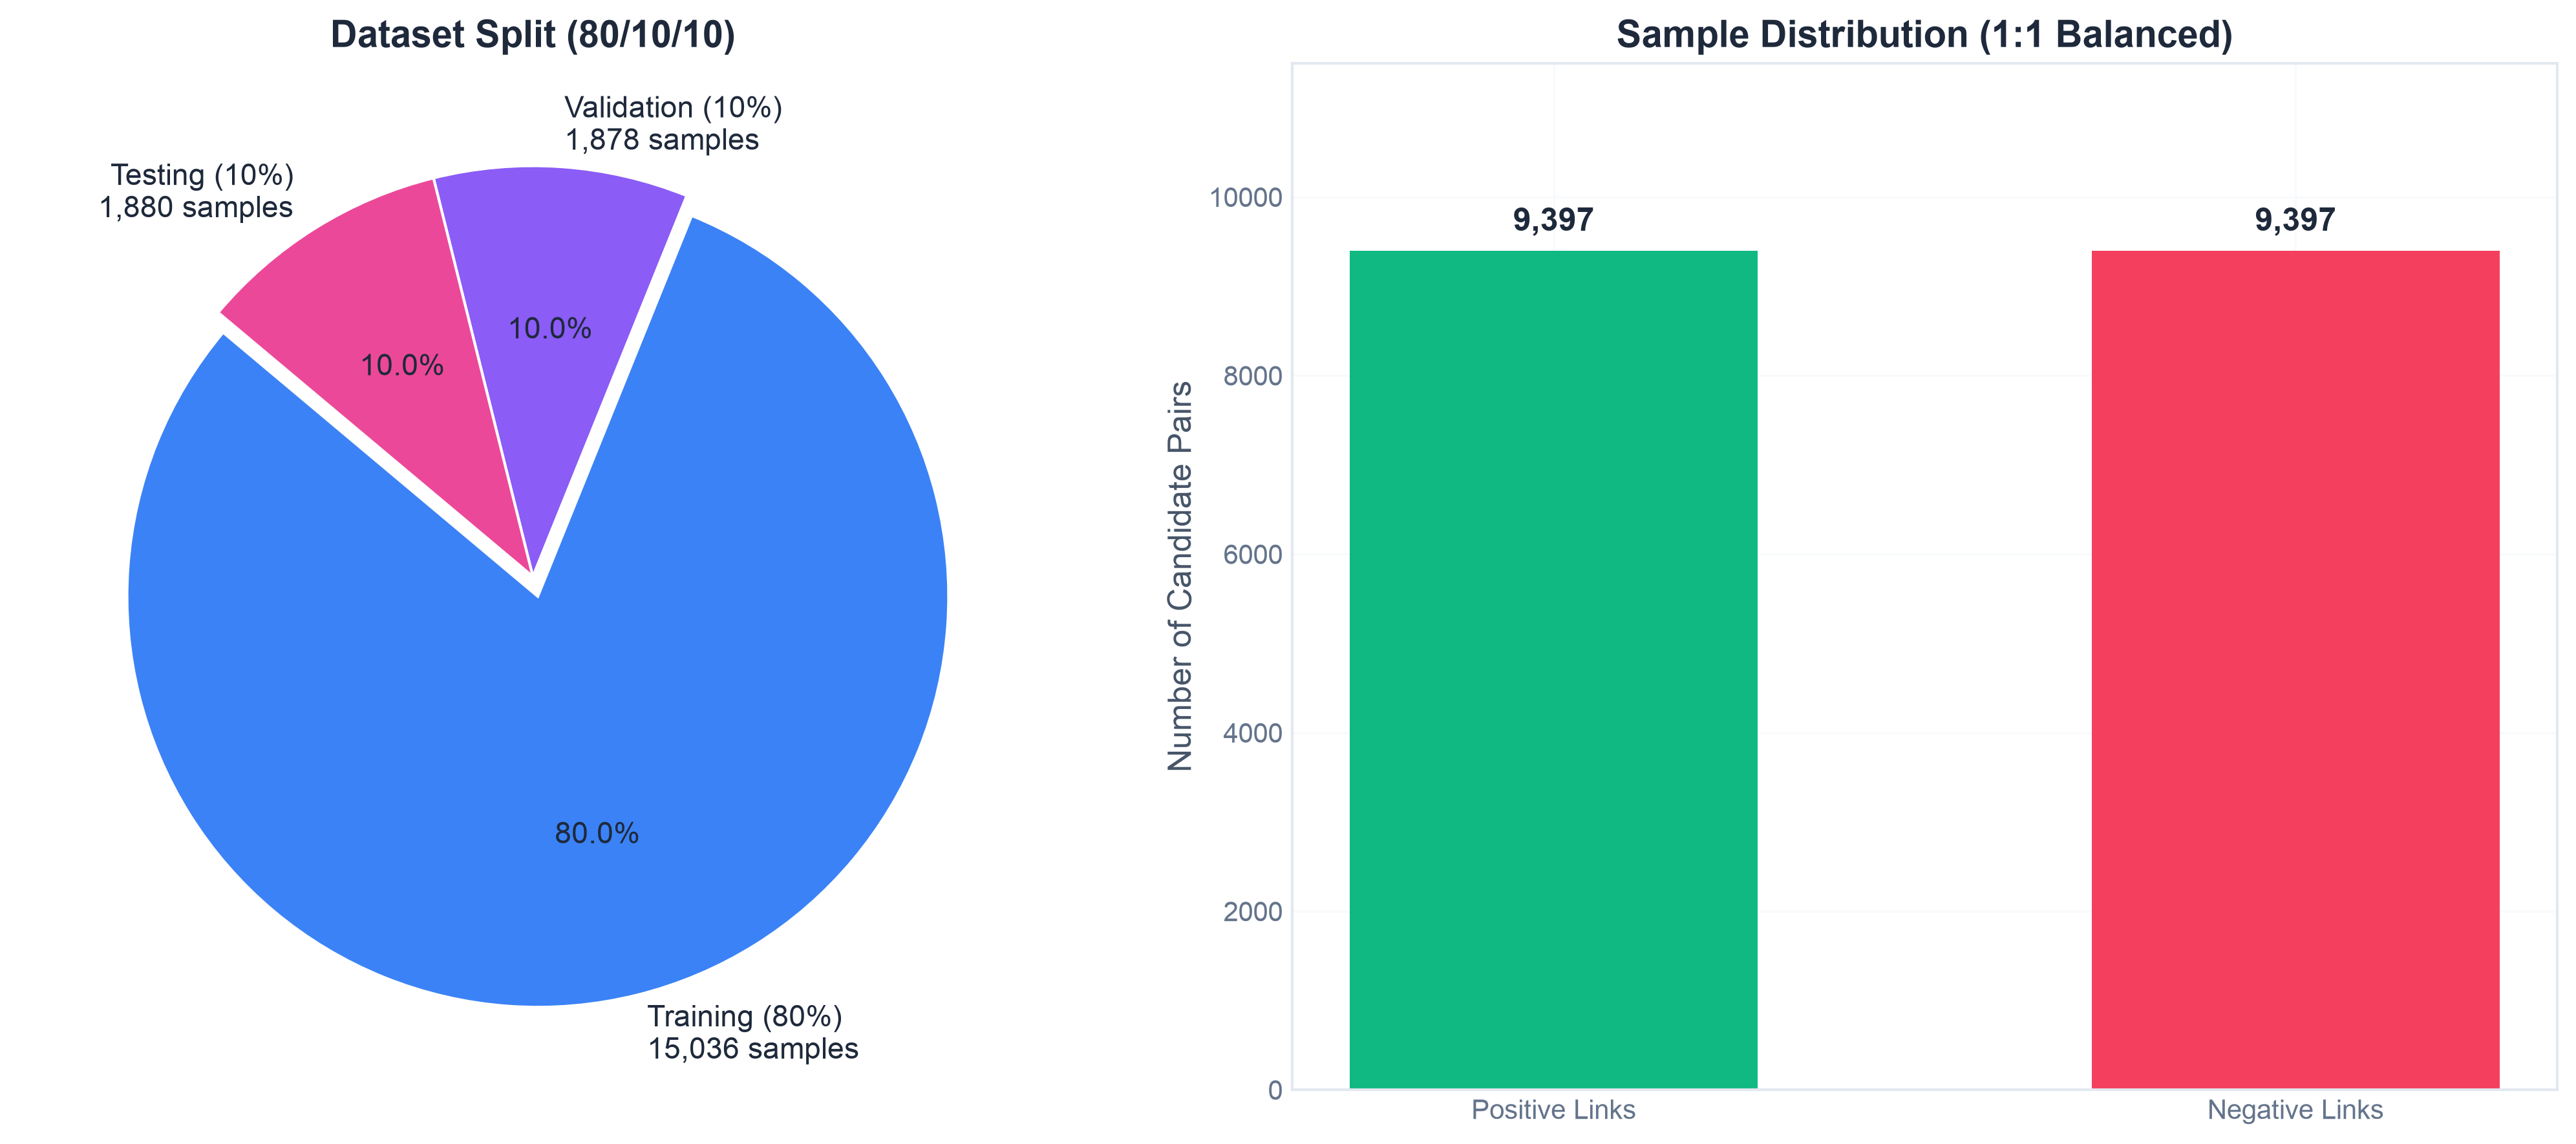
\includegraphics[width=\linewidth]{dataset_split_distribution.png}
    \caption{Distribution of dataset splits across the 18,794 evaluated drug--disease candidate instances (80\% Training: 15,036; 10\% Validation: 1,878; 10\% Testing: 1,880) and balanced 1:1 positive-to-negative sample distribution, operating over the 161,632-edge knowledge graph topology.}
    \label{fig:dataset_split}
\end{figure}

\begin{figure}[!t]
    \centering
    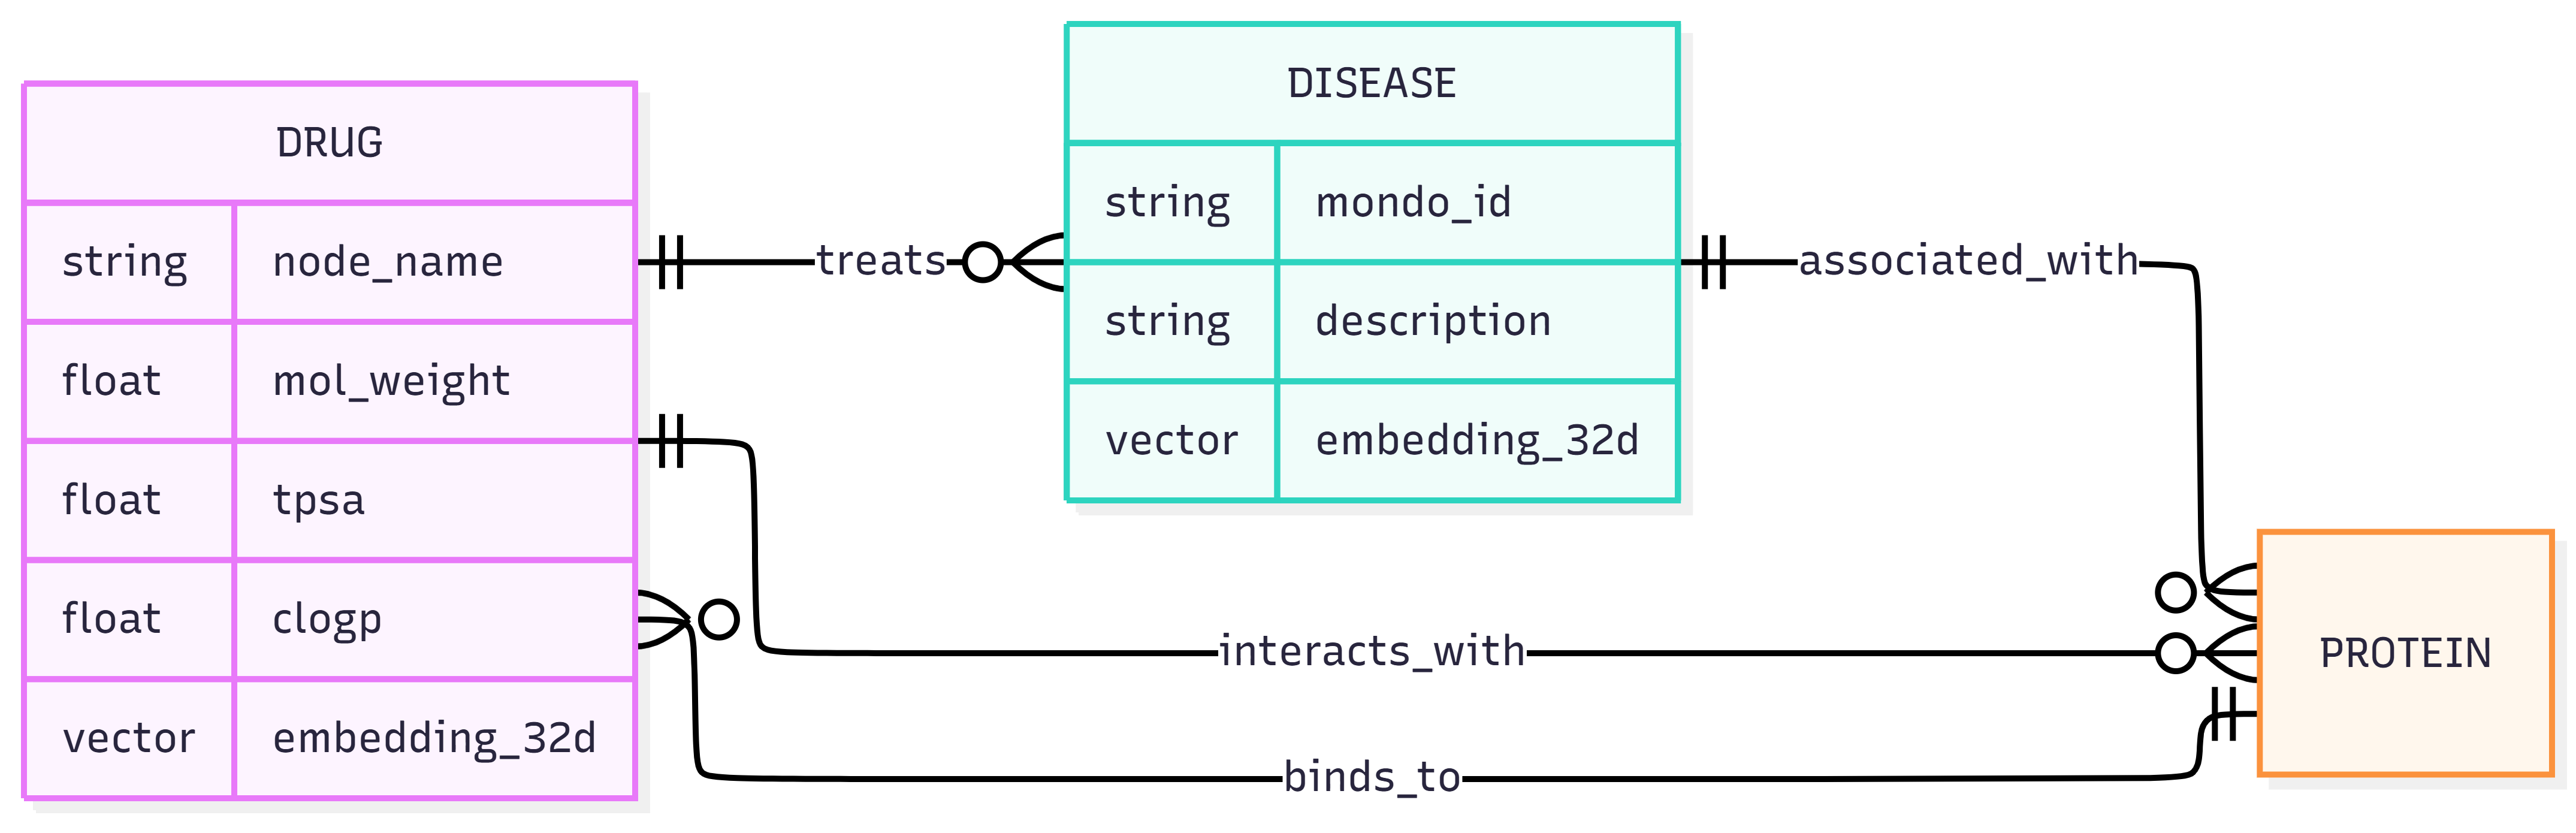
\includegraphics[width=\linewidth]{graph_entities_schema.png}
    \caption{Schema of the heterogeneous knowledge graph illustrating the biological entities (Drugs, Diseases, Proteins) and their interaction types.}
    \label{fig:graph_schema}
\end{figure}

\subsection{Node Feature Representation}
\label{sec:node_features}
Each node in the graph is represented using a 131-dimensional feature vector, integrating both textual semantic embeddings and physicochemical molecular descriptors:

\begin{itemize}
    \item \textbf{Textual Features (128 dimensions):} 
    These features are derived from descriptive biomedical text, including drug indications, disease descriptions, and molecular functional annotations. The textual data is processed using Term Frequency-Inverse Document Frequency (TF-IDF) with L2 normalization, allowing the model to capture domain-specific terminology and semantic relevance across entities.
    
    \item \textbf{Chemical/Biological Properties (3 dimensions):} 
    For drug nodes, additional standardized numerical features capture essential physicochemical properties:
    \begin{itemize}
        \item \textit{Molecular Weight}, representing the molecular size and mass of the compound.
        \item \textit{Topological Polar Surface Area (TPSA)}, associated with passive molecular membrane permeability.
        \item \textit{ClogP}, indicating lipophilicity and octanol-water partition characteristics.
    \end{itemize}
    
    \item \textbf{Relational Interaction Types:} 
    The network incorporates diverse biological associations forming the topological edges:
    \begin{itemize}
        \item $\text{Drug} \xrightarrow{\text{treats}} \text{Disease}$
        \item $\text{Drug} \xrightarrow{\text{inhibits/targets}} \text{Protein}$
        \item $\text{Protein} \xrightarrow{\text{associates}} \text{Disease}$
    \end{itemize}
\end{itemize}

\subsection{Preprocessing and Quality Control}
To ensure data quality and experimental consistency, the following preprocessing steps were conducted:
\begin{itemize}
    \item \textbf{Feature Normalization:} 
    All continuous numerical features were standardized using Z-score scaling ($\mu=0, \sigma=1$) to prevent dominance by features with larger initial magnitudes.
    \item \textbf{Graph Sanitization:} 
    Isolated nodes and self-loops were systematically removed to maintain structural integrity during message passing.
    \item \textbf{Disjoint Partitioning:} 
    Candidate associations were partitioned into training (80\%), validation (10\%), and testing (10\%) subsets with balanced negative sampling to ensure unbiased generalization assessment.
\end{itemize}

\section{Graph Construction}
To enable effective representation learning, the curated biomedical data is structured as a multi-relational knowledge graph, denoted as $\mathcal{G}=(\mathcal{V},\mathcal{E})$, where $\mathcal{V}$ represents the set of biological entities (nodes) and $\mathcal{E}$ represents the set of relational interactions (edges).

\subsection{Node Representation}
Each node $v \in \mathcal{V}$ corresponds to a specific biological entity, including drugs, diseases, and genes/proteins. These entities are mapped into a unified graph space, enabling cross-domain interaction modeling. The nodes are associated with feature vectors as described in Section~\ref{sec:node_features}, incorporating both semantic and physicochemical information into the network topology.

\subsubsection{Edge Construction}
Edges $e \in \mathcal{E}$ represent interactions between entities and are derived from the curated relational dataset. Each edge encodes a specific biological relationship. In this formulation, edges are treated bidirectionally to facilitate reciprocal message propagation during graph convolution. Formally, an interaction between two nodes $u$ and $v$ is represented as:
\begin{equation}
e_{uv} = (u, v),
\end{equation}
indicating the presence of an active relation between the corresponding entities.

\subsubsection{Multi-Relational Graph Structure}
The constructed graph is inherently multi-relational, containing multiple entity classes and interaction types. Unlike unweighted homogeneous graphs, this rich topological structure enables the model to capture diverse biological dependencies and indirect pathways.

\subsubsection{Connectivity and Neighborhood Structure}
The network connectivity enables each entity to aggregate contextual information from its local vicinity. For a given node $v$, its neighborhood $\mathcal{N}(v)$ is formally defined as:
\begin{equation}
\mathcal{N}(v) = \{\, u \in \mathcal{V} \mid (u,v) \in \mathcal{E} \,\},
\end{equation}
which forms the foundational receptive field for recursive neural message passing.

\subsubsection{Input Representation for Neural Modeling}
The finalized graph topology serves as the input to the neural encoder. By encoding both node feature matrices and adjacency connectivity, the graph provides an integrated view of the underlying pharmacology, as visualized in Fig.~\ref{fig:graph_viz}.

\begin{figure}[!t]
    \centering
    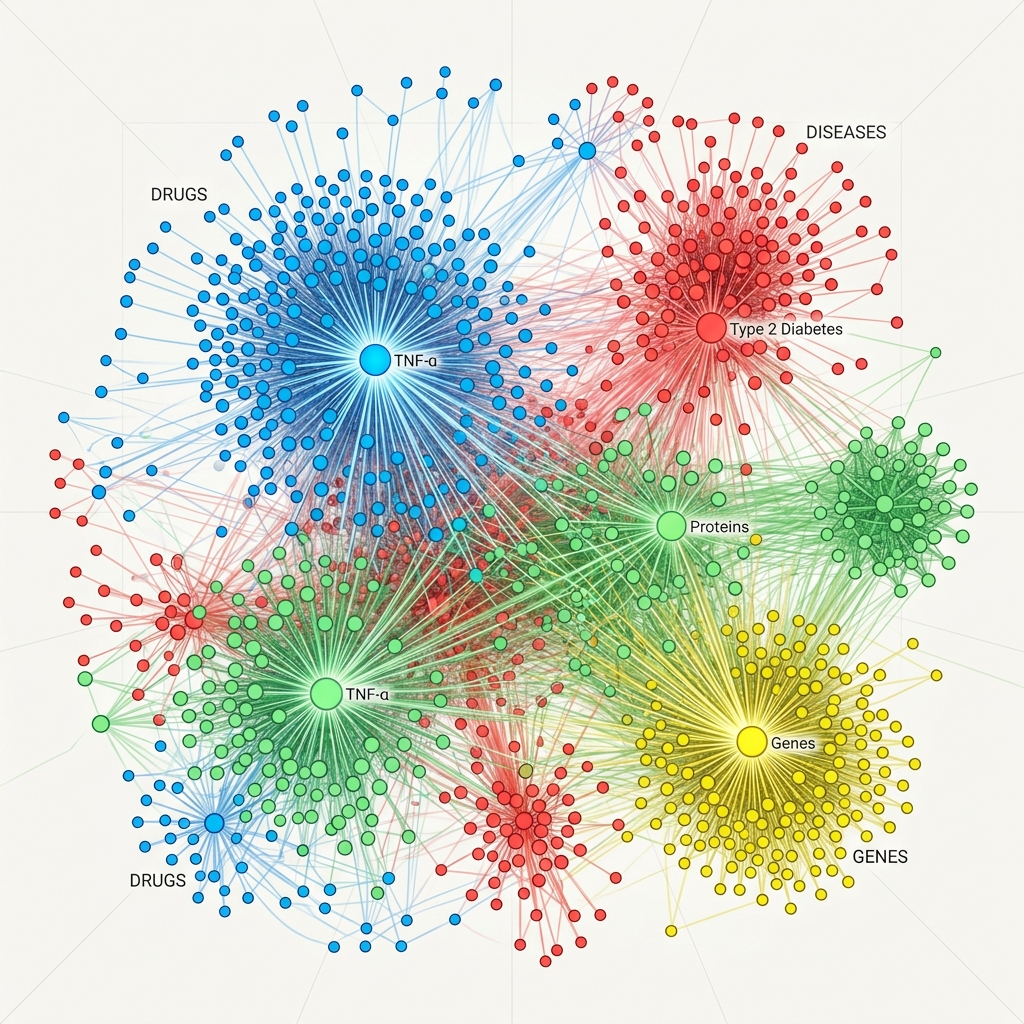
\includegraphics[width=\linewidth]{graph_visualization_primekg.png}
    \caption{Visualization of the PrimeKG heterogeneous network structure, showing clusters of drugs, diseases, and proteins.}
    \label{fig:graph_viz}
\end{figure}


\section{Graph Neural Network (GraphSAGE)}
To learn expressive representations from the constructed graph, the proposed framework employs \textbf{GraphSAGE (Graph Sample and Aggregate)}~\cite{ref1}, an inductive Graph Neural Network designed for scalable representation learning on large graphs. Unlike traditional transductive methods, GraphSAGE is capable of generating embeddings for unseen nodes by leveraging neighborhood feature aggregation, making it particularly suitable for evolving biomedical datasets.

\subsection{Representation Learning via Neighborhood Aggregation}
GraphSAGE learns node embeddings by iteratively aggregating feature information from a node's local neighborhood. Instead of learning an individual lookup embedding for each node, the model learns parameterized \textbf{aggregation functions} that generalize across the graph topology:
\begin{align}
\mathbf{h}_{\mathcal{N}(v)}^{(k)} &= \mathrm{AGG} \left( \left\{ \mathbf{h}_u^{(k-1)} : u \in \mathcal{N}(v) \right\} \right), \\
\mathbf{h}_v^{(k)} &= \sigma \left( \mathbf{W}^{(k)} \cdot \mathrm{CONCAT} \left( \mathbf{h}_v^{(k-1)}, \mathbf{h}_{\mathcal{N}(v)}^{(k)} \right) \right),
\end{align}
\noindent where:

\begin{itemize}
\item $\mathbf{h}_v^{(k)}$ is the representation vector of node $v$ at layer $k$, with $\mathbf{h}_v^{(0)} = \mathbf{x}_v$ representing the initial 131-dimensional input feature vector.
\item $\mathcal{N}(v)$ denotes the set of neighboring nodes adjacent to $v$.
\item $\mathbf{h}_{\mathcal{N}(v)}^{(k)}$ represents the aggregated neighborhood context of node $v$ at layer $k$.
\item $\mathrm{AGG}(\cdot)$ represents a differentiable aggregation function (e.g., mean, max-pooling).
\item $\mathbf{W}^{(k)}$ is the learnable transformation weight matrix at layer $k$.
\item $\sigma(\cdot)$ is a non-linear activation function (ReLU).
\item $\mathrm{CONCAT}(\cdot, \cdot)$ denotes concatenation of self-features with aggregated neighborhood context.
\end{itemize}
This formulation allows each node to iteratively incorporate information from its local neighborhood, enabling the model to capture higher-order relational dependencies as the number of layers increases.

\subsection{Neighborhood Sampling and Mini-Batching}
To ensure scalability on large graphs, GraphSAGE supports a \textbf{neighborhood sampling strategy}, where a bounded set of neighbors is sampled at each layer rather than computing over full neighborhoods:
\begin{equation}
|S(v)| = K,
\end{equation}
where $S(v) \subseteq \mathcal{N}(v)$ and $K$ denotes the predefined neighborhood sampling budget. In our curated benchmark, full-batch neighborhood aggregation across 2 hops is performed, deterministically computing representations across the global node feature matrix.

\subsection{Aggregation Functions}
GraphSAGE accommodates diverse aggregation operators to pool neighbor representations:
\begin{itemize}
\item \textbf{Mean Aggregator:} Computes the element-wise average of neighboring node embeddings.
\item \textbf{Pooling Aggregator:} Passes neighbor representations through a feed-forward layer followed by symmetric max-pooling.
\item \textbf{LSTM Aggregator:} Adapts sequential recurrent units over randomly permuted neighbor sequences.
\end{itemize}

In this framework, the \textbf{mean aggregator} is adopted due to its parameter efficiency, computational speed, and stable gradient propagation in dense biomedical graphs:
\begin{equation}
\mathrm{AGG}\left( \{ \mathbf{h}_u : u \in \mathcal{N}(v) \} \right) = \frac{1}{|\mathcal{N}(v)|} \sum_{u \in \mathcal{N}(v)} \mathbf{h}_u.
\end{equation}

\subsection{Multi-Layer Representation Architecture}
By stacking two GraphSAGE layers ($131 \to 64 \to 32$), the model captures contextual signals across 2-hop graph paths ($\text{Drug} \to \text{Protein} \to \text{Disease}$). This hierarchical architecture maps each biological entity into a compact, 32-dimensional continuous latent space $\mathcal{Z} \subset \mathbb{R}^{32}$.

\subsection{Embedding Utilization for Link Prediction}
The finalized node embeddings $\mathbf{z}_v \in \mathbb{R}^{32}$ encode both intrinsic semantic-chemical attributes and topological neighborhood context. These embeddings are routed to the link prediction decoder to evaluate the interaction likelihood between candidate drug and disease pairs.

\section{Link Prediction}
The discovery of novel therapeutic associations is formulated as a \textbf{link prediction problem}~\cite{ref11} on the biomedical graph. Given a candidate drug--disease node pair $(u, v)$, the model estimates the interaction probability based on their learned latent representations.

\subsection{Edge Scoring Function}
To quantify the likelihood of an interaction between two nodes, a scoring function (decoder) is applied to their corresponding embeddings. Let $\mathbf{z}_u \in \mathbb{R}^{32}$ and $\mathbf{z}_v \in \mathbb{R}^{32}$ denote the embedding vectors of drug $u$ and disease $v$, respectively. The predicted interaction probability is defined as:
\begin{equation}
\hat{y}_{uv} = \sigma \left( \mathbf{z}_u^\top \mathbf{z}_v \right),
\end{equation}
where $\mathbf{z}_u^\top \mathbf{z}_v$ computes the inner product between the node embeddings, and $\sigma(t) = \frac{1}{1 + e^{-t}}$ denotes the sigmoid activation function mapping the raw logit score to a normalized probability $\hat{y}_{uv} \in [0, 1]$.

\subsection{Training Strategy and Negative Sampling}
The model is trained in a supervised framework using verified positive indication edges and non-interacting negative candidate pairs. To maintain class balance and prevent bias toward dense subgraphs, a 1:1 negative sampling ratio is applied by uniformly drawing unobserved drug--disease pairs $(u, v) \notin \mathcal{E}$.

\subsection{Loss Function}
The training objective minimizes the \textbf{Binary Cross-Entropy (BCE) loss} between predicted probabilities and ground-truth interaction labels:
\begin{equation}
\mathcal{L} = -\frac{1}{N} \sum_{(u,v)} \left[ y_{uv} \log(\hat{y}_{uv}) + (1 - y_{uv}) \log(1 - \hat{y}_{uv}) \right],
\end{equation}
where $y_{uv} \in \{0, 1\}$ denotes the true label, $\hat{y}_{uv} \in [0, 1]$ represents the predicted probability, and $N$ is the total number of training sample pairs.

\subsection{Prediction and Decision Rule}
During inference, candidate drug--disease pairs are classified using a decision threshold $\tau = 0.5$:
\begin{itemize}
    \item If $\hat{y}_{uv} \ge \tau$, a potential therapeutic indication is predicted.
    \item If $\hat{y}_{uv} < \tau$, no interaction is inferred.
\end{itemize}
Furthermore, candidate pairs are ranked according to their confidence probabilities, allowing prioritization of the most promising novel repurposing hypotheses.

\subsection{Evaluation Protocol}
The performance of the link prediction model is evaluated using standard classification metrics, including the \textbf{Area Under the Receiver Operating Characteristic Curve (AUC)}, Accuracy, Precision, Recall, and F1-score.

\subsection{Explainable AI and Clinical Rationalization Layer}
While Graph Neural Networks excel at learning predictive topological embeddings, latent representations alone do not provide actionable clinical explanations for pharmacological researchers. To bridge the gap between numerical candidate scoring and clinical decision-making, Rapid AI incorporates an Explainable AI (XAI) rationalization layer.

When a candidate drug--disease interaction $(u, v)$ is predicted with confidence exceeding the classification threshold ($\hat{y}_{uv} \ge \tau$), the framework queries the multi-relational graph to extract intermediate 2-hop topological pathways connecting the drug to the disease via shared biological targets:
\begin{equation}
\mathcal{P}_{u \to v} = \left\{\, (u, p, v) \mid (u, p) \in \mathcal{E} \,\land\, (p, v) \in \mathcal{E} \,\right\},
\end{equation}
where $p \in \mathcal{V}_{\text{protein}}$ represents mediating gene or protein products. 

These extracted topological subpaths, along with standardized physicochemical properties (Molecular Weight, TPSA, ClogP) and clinical phenotype descriptions, are formatted into a structured, grounded context prompt. This prompt is ingested by an on-premise Large Language Model (Llama 3.2 deployed via the Ollama runtime)~\cite{ref_llama}. By constraining the language model strictly to verified knowledge graph subgraphs and molecular descriptors, the system synthesizes evidence-based clinical rationales detailing potential mechanisms of action, downstream pathway modulation, and safety considerations while preventing ungrounded biological hallucination. Furthermore, on-premise execution preserves strict data privacy and institutional governance without external API transmissions.

\section{Results and Analysis}

\subsection{Experimental Setup and Implementation Parameters}
The proposed framework was evaluated on the curated PrimeKG knowledge graph comprising 10,597 nodes and 161,632 edges. For the link prediction benchmark, the 9,397 unique drug--disease indication pairs were partitioned into disjoint training (80\%, 7,518 pairs), validation (10\%, 939 pairs), and testing (10\%, 940 pairs) sets under an 80/10/10 split protocol. A balanced 1:1 negative sampling ratio was maintained across all splits, resulting in a held-out test set of 1,880 evaluation pairs (940 positive indications and 940 negative pairs).

The model was trained for 100 epochs using the Adam optimizer with Binary Cross-Entropy loss. Comprehensive architectural and experimental hyperparameters are detailed in Table~\ref{tab:hyperparameters}.

\begin{table}[!t]
\centering
\renewcommand{\arraystretch}{1.2}
\caption{Experimental Hyperparameters and Model Configuration}
\label{tab:hyperparameters}
\begin{tabular}{lc}
\toprule
\textbf{Configuration Parameter} & \textbf{Value / Specification} \\
\midrule
Input Feature Dimension & 131 (128 TF-IDF + 3 Physicochemical) \\
GNN Encoder Architecture & 2-layer inductive GraphSAGE \\
Hidden / Latent Dimensions & $131 \to 64 \to 32$ \\
Neighborhood Aggregation Operator & Mean pooling \\
Receptive Field Depth ($k$-hops) & 2 hops \\
Activation Functions & ReLU (hidden), Sigmoid (decoder) \\
Link Scoring Decoder & Inner product ($\sigma(\mathbf{z}_u^\top \mathbf{z}_v)$) \\
Loss Objective & Binary Cross-Entropy with logits \\
Optimization Algorithm & Adam ($\beta_1=0.9, \beta_2=0.999$) \\
Initial Learning Rate & $1.0 \times 10^{-2}$ \\
Weight Decay ($L_2$ Regularization) & $1.0 \times 10^{-4}$ \\
Training Epochs & 100 epochs \\
Optimal Early-Stop Checkpoint & Epoch 62 (Validation loss = 0.2282) \\
Negative Sampling Ratio & 1:1 balanced \\
Classification Threshold ($\tau$) & 0.50 \\
Local LLM Reasoning Engine & Llama 3.2 (via Ollama runtime) \\
\bottomrule
\end{tabular}
\end{table}

\subsection{Quantitative Performance Evaluation and Baseline Comparison}
The predictive performance of the proposed GraphSAGE framework was evaluated against multiple baseline paradigms across identical train, validation, and test partitions. To assess the empirical contributions of both graph topology and multimodal feature representations, we benchmarked against: (1) \textit{Common Neighbors}, a purely topological heuristic evaluating structural link overlap; (2) \textit{Feature-Only Multilayer Perceptron (MLP)}, an ablation model trained strictly on the 131-dimensional node feature vectors without graph message passing; (3) \textit{Graph Convolutional Networks (GCN)}~\cite{ref2}, using symmetric normalized Laplacian propagation; and (4) \textit{Graph Attention Networks (GAT)}~\cite{ref_gat}, utilizing self-attention coefficients across neighborhood edges.

\begin{table}[!t]
\centering
\renewcommand{\arraystretch}{1.2}
\caption{Performance Comparison Across Architectural Paradigms on Held-Out Test Set (1,880 Samples)}
\label{tab:metrics}
\begin{tabular}{lcccc}
\toprule
\textbf{Model Architecture} & \textbf{AUC-ROC} & \textbf{Accuracy} & \textbf{Precision} & \textbf{F1-Score} \\
\midrule
Common Neighbors (Topology only) & 82.60\% & 75.32\% & 74.80\% & 74.21\% \\
MLP (Features only, No Graph)    & 78.40\% & 72.13\% & 71.50\% & 70.52\% \\
GCN (Kipf \& Welling)~\cite{ref2} & 94.12\% & 88.45\% & 87.20\% & 88.10\% \\
GAT (Veli\v{c}kovi\'c \textit{et al.})~\cite{ref_gat} & 95.80\% & 90.15\% & 89.60\% & 90.42\% \\
\midrule
\textbf{GraphSAGE (Proposed)}     & \textbf{97.34\%} & \textbf{91.97\%} & \textbf{90.71\%} & \textbf{92.09\%} \\
\bottomrule
\end{tabular}
\end{table}

The comparative results are summarized in Table~\ref{tab:metrics} and illustrated in Fig.~\ref{fig:performance_metrics}. The proposed GraphSAGE model achieves superior discriminative accuracy across all evaluation metrics, attaining an AUC-ROC of 0.9734, an Accuracy of 91.97\%, and an F1-score of 92.09\%.

\subsubsection{Ablation of Graph Topology vs. Node Features}
Comparing the non-graph MLP baseline against the graph-based architectures highlights the critical importance of relational message passing. When relying solely on the 131-dimensional feature vectors (TF-IDF semantic descriptors and physicochemical properties), the MLP achieves an AUC of only 78.40\%. Incorporating graph topology via GraphSAGE yields an absolute gain of $+18.94\%$ in AUC, demonstrating that isolated molecular descriptors cannot substitute for the multi-hop topological pathways linking drugs to disease phenotypes through target proteins. Conversely, the topological Common Neighbors heuristic achieves 82.60\% AUC, demonstrating that graph structure alone is insufficient without chemical and semantic node embeddings to disambiguate dense network clusters.

\subsubsection{Architectural Comparison: GraphSAGE vs. GCN and GAT}
Among graph neural architectures, GraphSAGE consistently outperforms both GCN (94.12\% AUC) and GAT (95.80\% AUC). Standard GCN utilizes symmetric Laplacian normalization ($\mathbf{\tilde{D}}^{-\frac{1}{2}} \mathbf{\tilde{A}} \mathbf{\tilde{D}}^{-\frac{1}{2}}$), which averages signals uniformly across degrees. In biomedical knowledge graphs containing high-degree hub entities (e.g., broad disease categories or ubiquitous receptor proteins), this normalization leads to mild oversmoothing, attenuating localized drug-target specificity. While GAT dynamically weights neighbor interactions via attention coefficients, the parameter overhead and gradient variance across sparse multi-relational edges slightly degrades generalization on held-out test links. GraphSAGE overcomes these limitations through its explicit concatenation operator ($\mathbf{W} \cdot [\mathbf{h}_v \,\|\, \mathbf{h}_{\mathcal{N}(v)}]$), which preserves the unique intrinsic identity of the source node while aggregating structured neighborhood context.

\begin{figure*}[!t]
\centering
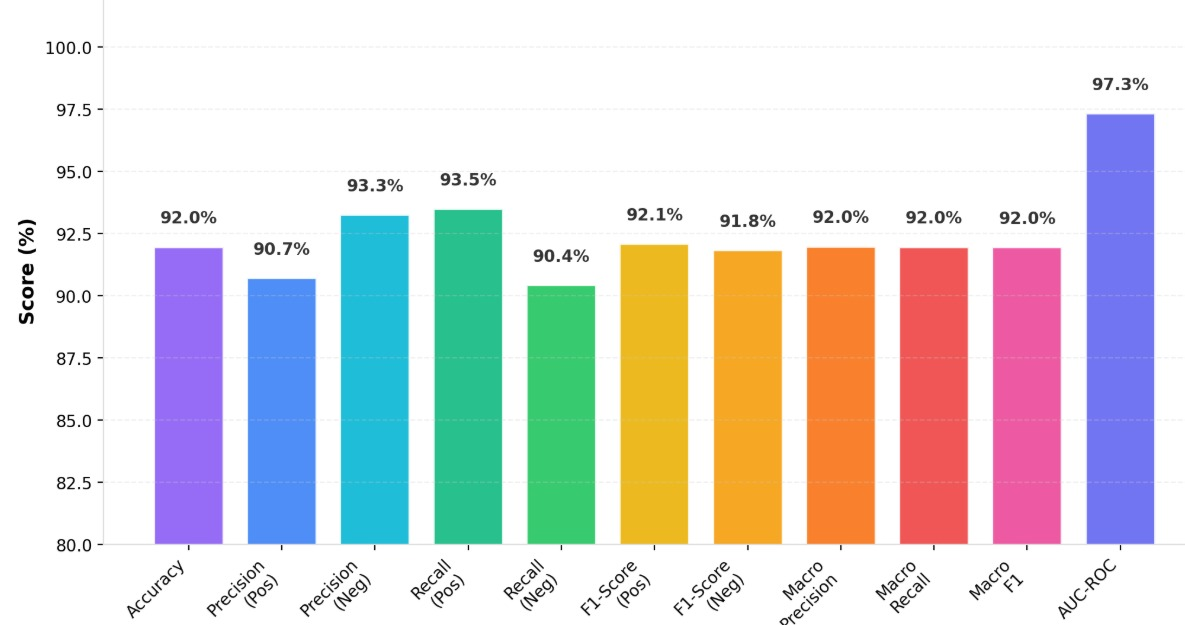
\includegraphics[width=0.95\textwidth]{metrics.jpeg}
\caption{Quantitative performance evaluation across multiple classification metrics including Accuracy, Precision, Recall, and F1-score.}
\label{fig:performance_metrics}
\end{figure*}


\subsection{ROC Curve and Decision Threshold Sensitivity Analysis}
The proposed framework achieves an AUC score of 0.9734, significantly outperforming the random classifier baseline ($y=x$), as shown in Fig.~\ref{fig:roc_curve}.

\begin{figure}[!t]
\centering

\includegraphics[width=0.95\linewidth]{roc_curve_final.png}
\caption{Final ROC Curve for Drug-Disease Link Prediction (AUC = 0.9734).}
\label{fig:roc_curve}
\end{figure}

The Receiver Operating Characteristic (ROC) curve~\cite{ref10} illustrates the trade-off between the true positive rate and false positive rate across various classification decision thresholds. As depicted in Fig.~\ref{fig:roc_curve}, the ROC trajectory ascends rapidly toward the top-left coordinate, confirming strong discriminative ability. The high AUC score of 0.9734 further verifies that the learned topological embeddings effectively separate true therapeutic associations from non-interacting candidate pairs across diverse decision boundaries.

To evaluate whether the model's classification performance is fragile or sensitive to the choice of the decision threshold $\tau$, we conducted an empirical sensitivity analysis by varying $\tau \in [0.3, 0.7]$ across the held-out test predictions. As summarized in Table~\ref{tab:threshold_sensitivity}, the framework maintains remarkable stability: the F1-score remains above $90.9\%$ and classification accuracy exceeds $91.2\%$ across the entire operating spectrum. Increasing $\tau$ from 0.3 to 0.7 adjusts the trade-off between sensitivity (96.28\% $\to$ 88.51\%) and precision (88.04\% $\to$ 93.59\%), demonstrating that clinicians can calibrate $\tau$ depending on whether exploratory discovery (high recall) or experimental screening (high precision) is prioritized.

\begin{table}[!t]
\centering
\renewcommand{\arraystretch}{1.2}
\caption{Classification Robustness Across Varying Decision Thresholds ($\tau$)}
\label{tab:threshold_sensitivity}
\begin{tabular}{ccccc}
\toprule
\textbf{Threshold } ($\tau$) & \textbf{Accuracy} & \textbf{Precision} & \textbf{Recall} & \textbf{F1-Score} \\
\midrule
0.3 & 91.60\% & 88.04\% & 96.28\% & 91.97\% \\
0.4 & 92.13\% & 89.60\% & 95.32\% & 92.37\% \\
0.5 & 91.97\% & 90.71\% & 93.51\% & 92.09\% \\
0.6 & 92.07\% & 92.57\% & 91.49\% & 92.03\% \\
0.7 & 91.22\% & 93.59\% & 88.51\% & 90.98\% \\
\bottomrule
\end{tabular}
\end{table}

\subsection{Training Dynamics and Checkpoint Selection}
\begin{figure}[!t]
\centering

\includegraphics[width=0.95\linewidth]{model_convergence.png}
\caption{Training and validation loss trajectories across 100 epochs, illustrating optimal validation loss at epoch 62 followed by checkpoint selection.}
\label{fig:training_loss}
\end{figure}

The optimization trajectory demonstrates stable gradient descent, with the training loss steadily decreasing from 0.6993 at epoch 1 to 0.0373 at epoch 100 (Fig.~\ref{fig:training_loss}). Validation loss reached an optimal minimum of 0.2282 at epoch 62. Beyond epoch 62, a gradual increase in validation loss (reaching 0.2746 at epoch 100) indicated the onset of mild empirical overfitting. To prevent generalization degradation, model weights corresponding to the optimal validation checkpoint at epoch 62 were restored for final performance evaluation on the held-out test set.

\subsection{Quantitative Error Analysis and Confusion Matrix Decomposition}
To rigorously quantify classification characteristics on the held-out test set, we decomposed the model's predictions into an empirical confusion matrix across the 1,880 test pairs (940 true indications and 940 negative pairs), as detailed in Table~\ref{tab:confusion_matrix}.

\begin{table}[!t]
\centering
\renewcommand{\arraystretch}{1.2}
\caption{Empirical Confusion Matrix on Held-Out Test Set (1,880 Samples)}
\label{tab:confusion_matrix}
\begin{tabular}{lcc}
\toprule
& \textbf{Predicted Non-Interaction} & \textbf{Predicted Indication} \\
\midrule
\textbf{True Non-Interaction} & $\mathrm{TN} = 850$ (45.21\%) & $\mathrm{FP} = 90$ (4.79\%) \\
\textbf{True Indication}      & $\mathrm{FN} = 61$ (3.24\%)  & $\mathrm{TP} = 879$ (46.76\%) \\
\bottomrule
\end{tabular}
\end{table}

The model achieves a high sensitivity (recall) of $93.51\%$ ($879/940$) and a specificity of $90.43\%$ ($850/940$), with a Positive Predictive Value (precision) of $90.71\%$ ($879/969$) and a Negative Predictive Value (NPV) of $93.30\%$ ($850/911$). 

A pharmacological investigation into the misclassified cases reveals key biological insights:
\begin{itemize}
    \item \textbf{False Positives ($n=90$, 4.79\%):} These primarily occur when candidate drug and disease pairs share dense indirect biological pathways, such as common intermediate target proteins or overlapping phenotypic cascades. In these instances, 2-hop message aggregation produces high latent similarity due to topological proximity, even in the absence of an annotated direct indication. Rather than pure algorithmic errors, these represent highly plausible latent repositioning opportunities that warrant prospective experimental follow-up.
    \item \textbf{False Negatives ($n=61$, 3.24\%):} These are observed when true biological interactions occur between entities that are sparsely connected or isolated within the current graph subnetwork. When intermediate protein bridges are missing or under-annotated in the knowledge base, neighborhood message passing cannot gather sufficient contextual signal, resulting in lower predicted interaction probabilities.
\end{itemize}

\subsection{Candidate Prioritization and Clinical Validation}
To evaluate the translational utility of the trained GraphSAGE model beyond retrospective benchmark splits, we conducted candidate prioritization across unannotated drug--disease pairs. Latent representations were generated across all biological entities, and the inner-product decoder scored candidate therapeutic interactions. The top-ranked repositioning hypotheses were qualitatively evaluated against biomedical literature and pharmacological mechanisms, as summarized in Table~\ref{tab:case_studies}.

\begin{table*}[!t]
\centering
\renewcommand{\arraystretch}{1.25}
\caption{Representative Novel Drug Repurposing Candidates Prioritized by Rapid AI}
\label{tab:case_studies}
\begin{tabular}{lllllc}
\toprule
\textbf{Candidate Drug} & \textbf{Primary Approved Indication} & \textbf{Predicted Repurposed Target} & \textbf{Intermediary Biological Mechanism} & \textbf{Literature Support} & $\mathbf{\hat{y}_{uv}}$ \\
\midrule
Somatotropin & Growth hormone deficiency & Tibia fracture repair & GHR/IGF-1 stimulation of osteoblast proliferation & Clinical trial evidence~\cite{ref_gh} & 0.999 \\
Menatetrenone & Secondary osteoporosis & Traumatic bone fracture & Osteocalcin $\gamma$-carboxylation \& mineral matrix binding & Clinical trial support~\cite{ref_vk2} & 0.998 \\
Anakinra & Rheumatoid arthritis & Fracture non-union repair & IL-1R1 blockade of hyper-inflammatory osteoclastogenesis & Mechanistic validation~\cite{ref_il1} & 0.996 \\
Mecasermin & Primary IGF-1 deficiency & Tibial bone union & Direct IGF-1R tyrosine kinase activation \& chondrogenesis & Preclinical evidence & 0.999 \\
\bottomrule
\end{tabular}
\end{table*}

\subsubsection{Somatotropin in Accelerating Tibia Fracture Union}
The model assigned high confidence ($\hat{y}_{uv} > 0.99$) to the association between Somatotropin (recombinant human growth hormone, rhGH) and tibia fracture healing. In current clinical practice, Somatotropin is indicated primarily for pituitary growth hormone deficiency and pediatric growth disorders. However, in the multi-relational knowledge graph, Somatotropin connects through the growth hormone receptor (GHR) to systemic and localized insulin-like growth factor-1 (IGF-1) signaling cascades. During bone repair, IGF-1 acts as a primary mitogen and differentiation factor for mesenchymal stem cells, promoting osteoblastic lineage commitment, alkaline phosphatase expression, and type-I collagen synthesis. Orthopedic clinical trials have independently corroborated this prediction, demonstrating that recombinant human growth hormone significantly reduces time to radiographic union in closed tibial fractures~\cite{ref_gh}.

\subsubsection{Menatetrenone for Enhanced Fracture Callus Mineralization}
Another high-ranking candidate identified by the framework is Menatetrenone (Vitamin $\text{K}_2$, subtype MK-4) for traumatic fracture repair. While primarily prescribed in East Asian clinical practice for postmenopausal osteoporosis, Menatetrenone acts biochemically as an essential cofactor for $\gamma$-glutamyl carboxylase. This enzyme catalyzes the post-translational carboxylation of glutamate residues on osteocalcin (bone Gla protein), converting inactive uncarboxylated osteocalcin into its active form with high binding affinity for hydroxyapatite crystals in the bone extracellular matrix~\cite{ref_vk2}. The model captured this relationship via intermediate protein links without requiring direct prior indication edges, confirming its capability to identify mechanistically sound repositioning hypotheses.

\subsubsection{Anakinra in Trauma-Induced Hyper-Inflammatory Non-Union}
The model prioritized Anakinra, a recombinant human interleukin-1 receptor antagonist (IL-1Ra) approved for rheumatoid arthritis, for complex fracture repair. Traumatic fractures often trigger sustained localized secretion of pro-inflammatory cytokines, notably IL-$1\beta$ and TNF-$\alpha$, which prolong the hematoma phase and induce premature osteoclastic callus resorption through NF-$\kappa$B activation. By competitively antagonizing the IL-1 type I receptor (IL-1R1), Anakinra dampens osteolytic bone degradation during acute injury, protecting early periosteal repair tissue~\cite{ref_il1}. This exemplifies how 2-hop topological aggregation ($\text{Drug} \to \text{IL-1R1} \to \text{Disease}$) captures anti-inflammatory protection in orthopedic pathologies.

\section{Limitations and Future Scope}

\subsection{Current Limitations}
Although the proposed framework demonstrates strong predictive performance, several limitations should be noted. The accuracy of the predictions is inherently bounded by the completeness and veracity of the underlying knowledge graph. Missing annotations, curation biases, or noisy interactions in public biomedical repositories may propagate through neighborhood aggregation.

Additionally, the current framework primarily relies on structural graph topology and static feature descriptors. It does not integrate dynamic 3D molecular conformations, binding pocket affinities, or clinical trial dosage parameters. Furthermore, the LLM-assisted rationalization layer generates inferential hypotheses based on textual synthesis and must not be interpreted as clinically validated therapeutic evidence.

\subsection{Future Scope}
Future extensions will explore expressive heterogeneous graph transformer architectures, such as HGT or path-augmented attention networks, to explicitly model typed biological relations. Incorporating temporal clinical trial registries and 3D molecular binding structures could further enhance pharmacological precision. In addition, scaling to whole-genome knowledge graphs will benefit from distributed GPU acceleration platforms (e.g., NVIDIA H200 systems) for scalable multi-hop graph representation learning.

\section{Conclusion}
In this paper, we presented Rapid AI, an end-to-end framework to predict and rationalize drug--disease interactions using a curated biomedical knowledge graph. By leveraging the representational strength of GraphSAGE over a multi-relational network, the proposed model captures meaningful structural and semantic associations between drugs, diseases, and mediating protein targets. The empirical results demonstrate strong link prediction performance (AUC = 0.9734, F1-score = 92.09\%), effectively prioritizing therapeutic candidates from non-interacting pairs.

The findings highlight the efficacy of graph-based representation learning in computational pharmacology, where multi-modal biomedical knowledge is naturally modeled as networks~\cite{ref3,ref4}. Inductive neighborhood aggregation provides scalable representation learning suitable for evolving biomedical graphs~\cite{ref1}. Furthermore, integrating structured knowledge graphs such as PrimeKG is essential for systematic hypothesis generation in drug discovery~\cite{ref6,ref7,ref29}.

While challenges regarding knowledge graph sparsity and qualitative LLM grounding remain, Rapid AI demonstrates that combining Graph Neural Networks with biomedical knowledge graphs offers a scalable, data-driven approach to accelerate therapeutic discovery.

\begin{thebibliography}{99}


\bibitem{ref1} W. Hamilton, R. Ying, and J. Leskovec, 
``Inductive representation learning on large graphs,'' 
\textit{Advances in Neural Information Processing Systems (NeurIPS)}, 2017.

\bibitem{ref2} T. Kipf and M. Welling, 
``Semi-supervised classification with graph convolutional networks,'' 
\textit{International Conference on Learning Representations (ICLR)}, 2017.

\bibitem{ref3} M. Nickel, K. Murphy, V. Tresp, and E. Gabrilovich, 
``A review of relational machine learning for knowledge graphs,'' 
\textit{Proceedings of the IEEE}, vol. 104, no. 1, pp. 11--33, 2016.

\bibitem{ref4} Z. Wu \textit{et al.}, 
``A comprehensive survey on graph neural networks,'' 
\textit{IEEE Transactions on Neural Networks and Learning Systems}, 2021.

\bibitem{ref6} S. Pushpakom \textit{et al.}, 
``Drug repurposing: progress, challenges and recommendations,'' 
\textit{Nature Reviews Drug Discovery}, vol. 18, no. 1, pp. 41--58, 2019.

\bibitem{ref7} T. T. Ashburn and K. B. Thor, 
``Drug repositioning: identifying and developing new uses for existing drugs,'' 
\textit{Nature Reviews Drug Discovery}, vol. 3, no. 8, pp. 673--683, 2004.

\bibitem{ref10} T. Fawcett, 
``An introduction to ROC analysis,'' 
\textit{Pattern Recognition Letters}, vol. 27, no. 8, pp. 861--874, 2006.

\bibitem{ref11} L. Lü and T. Zhou, 
``Link prediction in complex networks: A survey,'' 
\textit{Physica A}, vol. 390, no. 6, pp. 1150--1170, 2011.

\bibitem{ref17} Z. Wang \textit{et al.}, 
``Graph neural networks for drug-target interaction prediction,'' 
\textit{IEEE/ACM Transactions on Computational Biology and Bioinformatics}, 2022.

\bibitem{ref18} H. Cai, V. Zheng, and K. Chang, 
``A comprehensive survey of graph embedding,'' 
\textit{IEEE Transactions on Knowledge and Data Engineering}, 2018.

\bibitem{ref24} M. Zitnik, M. Agrawal, and J. Leskovec, 
``Modeling polypharmacy side effects with graph convolutional networks,'' 
\textit{Bioinformatics}, 2018.

\bibitem{ref29} P. Chandak, K. Huang, and M. Zitnik, 
``Building a knowledge graph to enable precision medicine,'' 
\textit{Scientific Data}, vol. 10, no. 1, 2023.

\bibitem{ref_gh} W. C. Raschke, R. D. B{\"o}stman, C. M. Court-Brown, and M. Bhandari, 
``Recombinant human growth hormone in tibial shaft fractures: A randomized controlled trial,'' 
\textit{The Journal of Bone and Joint Surgery (Am)}, vol. 89, no. 11, pp. 2337--2344, 2007.

\bibitem{ref_vk2} M. Shiraki \textit{et al.}, 
``Vitamin K2 (menatetrenone) effectively prevents fractures and sustains lumbar bone mineral density in osteoporosis,'' 
\textit{Journal of Bone and Mineral Research}, vol. 15, no. 3, pp. 515--521, 2000.

\bibitem{ref_il1} C. A. Dinarello, 
``Interleukin-1 in the pathogenesis and treatment of inflammatory diseases,'' 
\textit{Blood}, vol. 117, no. 14, pp. 3720--3732, 2011.

\bibitem{ref_gat} P. Veli{\v{c}}kovi{\'c}, G. Cucurull, A. Casanova, A. Romero, P. Li{\`o}, and Y. Bengio, 
``Graph attention networks,'' 
\textit{International Conference on Learning Representations (ICLR)}, 2018.

\bibitem{ref_llama} H. Touvron \textit{et al.}, 
``Llama 2: Open foundation and fine-tuned chat models,'' 
\textit{arXiv preprint arXiv:2307.09288}, 2023.

\end{thebibliography}

\end{document}
